\chapter{电磁感应}\label{chp:electromagnetic_induction}
\section{电磁感应现象}
在奥斯特发现电流的磁效应以后,人们自然想到:既然电流能够产生磁场,反过来磁场是不是也能产生电流呢?
最容易产生的设想是把导线绕在磁铁上,导线两端接上电流表,构成一个闭合电路,看看能不能产生电流。
法拉第就是这样开始来研究的,结果发现电流表的指针并不偏转。
换用强的电磁铁,或者换用更灵敏的电流表,结果还是一样,没有电流。
怎样才能获得电流呢?下面用实验来研究这个问题。

\subsection*{实验一}
如\cref{fig:2-1} 所示,如果让导体 $AB$ 在磁场中向左或向右运动,电流表的指针就发生偏转,表明电路中有了电流。
导体 $AB$ 停下来,电流也就消失了。
这就是说,闭合电路
\begin{figure}
  \includegraphics{2-1.pdf}
  \caption{}\label{fig:2-1}
\end{figure}
的一部分导体相对于磁场运动时,电路中就有电流产生。
但是,如果让导体 $AB$ 在磁场中向上或向下运动,电路中却不产生电流。
怎样分析上述现象呢?
我们知道,磁场可以用磁力线形象地表示出来,有了磁力线的概念,就容易分析上述现象了。
导体 $AB$ 向左或向右运动时切割磁力线,向上或向下运动时不切割磁力线。可见,闭合电路的一部分导体做切割磁力线的运动时,电路中才有电流产生。

在这个实验中,导体 $AB$ 运动,如果导体不动,让磁场运动,会不会在电路中产生电流呢?让我们做下面的实验。

\subsection*{实验二}
\medskip\noindent
\begin{minipage}{0.62\linewidth}\parindent2em
如\cref{fig:2-2} 所示,把一个磁铁插入螺线管,或者从螺线管里拿出来,可以看到,磁铁相对于螺线管运动的时候,电流表的指针发生偏转,表明螺线管电路中有了电流。
如果保持磁铁在螺线管中不动,或者让二者以同一速度运动,即保持相对静止,螺线管中就没有电流了。
在这个实验中,磁铁相对于螺线管运动时,螺线管的导线切割磁力线。
可见,不论是导体运动,还是磁场运动,只要闭合电路的一部分导体切割磁力线,电路中就有电流产生。
\end{minipage}\hfill
\begin{minipage}{0.33\linewidth}\centering
\begin{figurehere}
\includegraphics{2-2.pdf}
\caption{}\label{fig:2-2}
\end{figurehere}
\end{minipage}

\medskip
闭合电路的一部分导体切割磁力线时,穿过闭合电路的磁力线条数发生变化。
由此提示我们:如果导体和磁场不发生相对运动,而让穿过闭合电路的磁场发生变化,会不会在电路中产生电流呢?
为了研究这个问题,我们做下面的实验。

\subsection*{实验三}
如\cref{fig:2-3} 所示,把螺线管 $B$ 套在螺线管 $A$ 的外面,合上电键给螺线管 $A$ 通电时,电流表的指针发生偏转,螺线管 $B$ 中有了电流。
当螺线管 $A$ 中的电流达到稳定时,螺线管 $B$ 中的电流消失。
打开电键使螺线管 $A$ 断电时,螺线管 $B$ 中也有电流产生。
如果用变阻器来改变电路中的电阻,使螺线管 $A$ 中的电流强度发生变化,螺线管 $B$ 中也有电流产生。
在这个实验中,螺线管 $B$ 处在螺线管 $A$ 的磁场中,当 $A$ 通电和断电时,或者使 $A$ 中的电流强度发生变化时,$A$ 的磁场随着发生变化。
因此,这个实验表明:在导体和磁场不发生相对运动的情况下,只要闭合电路中的磁场发生变化,因而穿过闭合电路的磁力线条数发生变化,闭合电路中就有电流产生。
\begin{figure}
\includegraphics{2-3.pdf}
\caption{}\label{fig:2-3}
\end{figure}

\subsection*{结论}
不论是闭合电路的一部分导体做切割磁力线的运动,还是闭合电路中的磁场发生变化,穿过闭合电路的磁力线条数都发生变化,这时闭合电路中就有电流产生。
我们在\cref{chp:magnetic_field}学过磁通量的概念,磁通量表示的就是穿过某个面的磁力线条数。
这样,利用磁通量的概念,我们就可以总结出如下的结论:

\emph{不论用什么方法,只要穿过闭合电路的磁通量发生变化,闭合电路中就有电流产生}。这种利用磁场产生电流的现象叫做\Concept{电磁感应},产生的电流叫做\Concept{感生电流}。

电磁感应现象是法拉第经过十多年的实验研究,在 1831 年发现的。
这一重大发现进一步揭示了电和磁的密切联系,为后来麦克斯韦建立完整的电磁理论莫定了基础。
根据这一发现后来发明了发电机、变压器等电器设备,开辟了电能在生产和生活中广泛应用的途径。

\begin{Reading}{法拉第电磁感应的发现}
1820 年奥斯特发现了电流的磁效应后,法拉第仔细地分析了电流的磁效应,他认为,既然磁铁可以使靠近它的铁块具有磁性,静电荷可以使靠近它的导体带电,那么电流也应当使靠近它的线圈感生出电流。1
822 年法拉第在日记中记载着“把磁转变成电”的光辉思想。
后来法拉第对这一课题进行了系统的实验研究。

开始,法拉第认为:用强磁铁靠近导线,导线中就会产生稳恒电流。
法拉第企图用实验证实这个设想,结果未获成功。
但法拉第不怕困难,顽强奋战了十年,终于取得了重大突破,1831 年发现了电磁感应现象。
\begin{figurehere}
  \begin{minipage}{\linewidth}\centering
    \includegraphics{2-4.pdf}
    \caption{}\label{fig:2-4}
  \end{minipage}
\end{figurehere}

1831 年 8 月法拉第把两个线圈绕在一个铁环上(\cref{fig:2-4}),线圈 $A$ 接直流电源,线圈 $B$ 接电流表。
他发现,当线圈 $A$ 中的电流接通或断开时,线圈 $B$ 中就产生瞬时电流。
法拉第发现,铁环并不是必须的。
拿走铁环,再做这个实验,电磁感应现象仍然发生,只是线圈中的电流弱些。

法拉第怎样分析他的实验呢?他的思路大致如下:

第一,线圈 $B$ 除了处在通电线圈 $A$ 的磁场中,同 $A$ 没有别的联系,所以 $B$ 的感生电流只能由 $A$ 的磁场引起,这正是他探寻了十年的磁生电的现象。

第二,$A$ 中电流稳定因而周围磁场稳定时,$B$ 中没有感生电流,表明稳定的磁场不引起感生电流;只有当 $A$ 通电或断电,它的电流变化因而周围磁场变化时,$B$ 中才有感生电流,表明变化的磁场才能引起感生电流。

第三,磁场可以由磁力线形象地描绘,$B$ 所在处的磁场变化,也就是穿过线圈 $B$ 的磁力线条数变化,即磁通量发生变化。

所以,感生电流的产生条件,可以归结为穿过线圈的磁通量变化。

为了透彻研究电磁感应现象,法拉第还做了许多其他实验。
1831 年 11 月法拉第在所写的论文中把产生感生电流概括为五种情况:变化着的电流;变化着的磁场;运动的稳恒电流;运动的磁铁;在磁场中运动的导体。
法拉第按照他的力线理论把产生感生电流的条件归结为:变化的磁力线能使导体中产生感生电流。
\end{Reading}

\begin{Practice}
\begin{question}
  \item 如\cref{fig:2-5} 所示,在磁场中有一个闭合的弹簧线圈,当\cref{fig:2-5a} 中人的双手离开后,线圈收缩(\cref{fig:2-5b}),线圈收缩时,其中是否有感生电流?为什么?
  \begin{figurehere}
    \begin{minipage}{\linewidth}\centering
      \nextfloat
    \begin{minipage}{0.45\linewidth}\centering
      \includegraphics{2-5a.pdf}
      \subcaption{}\label{fig:2-5a}
    \end{minipage}
    \begin{minipage}{0.45\linewidth}\centering
      \includegraphics{2-5b.pdf}
      \subcaption{}\label{fig:2-5b}
    \end{minipage}
    \caption{}\label{fig:2-5}
    \end{minipage}
  \end{figurehere}
  \item 在\cref{fig:2-6} 所示的匀强磁场中有一个线圈板,线圈平面垂直于磁力线,当线圈框在磁场中上下通动对,是否会在线圈框中引起感生电流?当线圈框在磁场中左右运动时,是否会在线圈框中引起感生电流?为什么?
  \begin{figurehere}
    \begin{minipage}[b]{0.48\linewidth}\centering
      \includegraphics{2-6.pdf}
      \caption{}\label{fig:2-6}
    \end{minipage}
    \begin{minipage}[b]{0.48\linewidth}\centering
      \includegraphics{2-7.pdf}
      \caption{}\label{fig:2-7}
    \end{minipage}
  \end{figurehere}
  \item 如\cref{fig:2-7} 所示,线圈在匀强磁场中绕 $OO'$ 轴转动时,线圈里是否有感生电流?为什么?
  \item 如\cref{fig:2-8} 所示,让闭合线圈由位置 1 通过一个匀强磁场运动到位置 2。线圈在运动过程中,什么时候有感生电流,什么时候没有感生电流?为什么?
  \begin{figurehere}
    \begin{minipage}[b]{0.48\linewidth}\centering
      \includegraphics{2-8.pdf}
      \caption{}\label{fig:2-8}
    \end{minipage}
    \begin{minipage}[b]{0.48\linewidth}\centering
      \includegraphics{2-9.pdf}
      \caption{}\label{fig:2-9}
    \end{minipage}
  \end{figurehere}
  \item 矩形线圈 $ABCD$ 位于通电直长导线附近(\cref{fig:2-9}),线圈跟导线同在一个平面内,且线圈的两个边与导线平行。在这个平面内,线圈远离导线平动时,线圈中有没有感生电流?线圈和导线都不动,当导线中的电流 $I$ 逐渐增大或减小时,线圈中有没有感生电流?为什么?
  \item 把一个铜环放在匀强磁场中,使环的平面与磁场的方向垂直(\cref{fig:2-10a})。如果使环沿着磁场的方向移动,铜环中是否产生感生电流?为什么?如果磁场是不均匀的(\cref{fig:2-10b}),是否产生感生电流?为什么?
  \begin{figurehere}
    \begin{minipage}{\linewidth}\centering
      \nextfloat
      \begin{minipage}{0.4\linewidth}\centering
        \includegraphics{2-10a.pdf}
        \subcaption{}\label{fig:2-10a}
      \end{minipage}
      \begin{minipage}{0.4\linewidth}\centering
        \includegraphics{2-10b.pdf}
        \subcaption{}\label{fig:2-10b}
      \end{minipage}
      \caption{}\label{fig:2-10}
    \end{minipage}
  \end{figurehere}
\end{question}
\end{Practice}


\section{感生电流的方向\texorpdfstring{\quad}{ }楞次定律}
在前一节的实验中,电流表的指针有时向右偏转,有时向左偏转,表示在不同情况下感生电流的方向是不同的。
怎样来确定感生电流的方向呢?

现在我们利用\cref{fig:2-2} 的实验来研究这个问题。

前一节我们利用磁通量的概念概括出了产生感生电流的条件,由此自然地想到,也要利用磁通量的概念来表达确定感生电流方向的规律。
当把磁铁的 $N$ 极移近或插入螺线管时(\cref{fig:2-11a}),穿过螺线管的磁通量增加。
从实验知道,这时感生电流的磁场方向跟磁铁的磁场方向相反,阻碍原来磁通量的增加。
当磁铁的 $N$ 极离开螺线管或者从中拔出时(\cref{fig:2-11b}),穿过螺线管的磁通量减少。
从实验知道,这时感生电流的方向跟\cref{fig:2-11a} 中的方向相反,它的磁场方向跟磁铁的磁场方向相同,阻碍原来磁通量的减少。
在其他电磁感应现象中,也有相同的规律。
凡是由磁通量的增加引起的感生电流,它所激发的磁场就阻碍原来磁通量的增加;凡是由磁通量的减少引起的感生电流,它所激发的磁场就阻碍原来磁通量的减少。
\begin{figure}
  \begin{minipage}[b]{0.4\linewidth}\centering
    \includegraphics{2-11a.pdf}
    \subcaption{}\label{fig:2-11a}
  \end{minipage}
  \begin{minipage}[b]{0.4\linewidth}\centering
    \includegraphics{2-11b.pdf}
    \subcaption{}\label{fig:2-11b}
  \end{minipage}
  \caption{}\label{fig:2-11}
\end{figure}

德国物理学家楞次(1804--1865)概括了各种实验结果,在 1834 年得到如下结论:

\emph{感生电流具有这样的方向,就是感生电流的磁场总要阻碍引起感生电流的磁通量的变化},这就是\Concept{楞次定律}。

我们知道,通电螺线管相当于条形磁铁,也有两个磁极。
如\cref{fig:2-11a} 所示,当磁铁的 $N$ 极移近螺线管时,利用安培定则可以知道,这时螺线管的上端是 $N$ 极,因而磁铁受到推斥,阻碍磁铁相对于螺线管的运动。
如\cref{fig:2-11b} 所示,当磁铁的 $N$ 极离开螺线管时,利用安培定则可以知道,这时螺线管的上端是 $S$ 极,因而磁铁受到吸引,也要阻碍磁铁相对于螺线管的运动。
总之,楞次定律的内容是:从磁通量变化的角度来看,感生电流总要阻碍磁通量的变化;从导体和磁场的相对运动的角度来看,感生电流总要阻碍相对运动。

利用楞次定律可以判断各种情况下感生电流的方向。

\section{楞次定律的应用}
应用楞次定律来判断感生电流的方向,首先要明确原来磁场的方向,以及穿过闭合电路的磁通量是增加还是减少,然后根据楞次定律确定感生电流的磁场方向,最后利用安培定则来确定感生电流的方向,下面用几个例子来说明怎样应用楞次定律。

\subsection*{应用之一}
现在来确定磁铁的 $S$ 极移近或离开螺线管时感生电流的方向。
如\cref{fig:2-12a} 所示,把磁铁的 $S$ 极移近螺线管时,原来的磁场方向向上,穿过螺线管的磁通量增加。
从楞次定律知道,感生电流要阻碍磁通量的增加,因此感生电流的磁场方向跟原来的磁场方向相反,即感生电流的磁场方向是向下的,如图中虚线所示。
知道了感生电流的磁场方向,利用安培定则就可以确定感生电流的方向。
如\cref{fig:2-12b} 所示,当磁铁的 $S$ 极离开螺线管时,原来的磁场方向向上,穿过螺线管的磁通量减少。
从楞次定律知道,感生电流要阻碍磁通量的减少,因此感生电流的磁场方向跟原来的磁场方向相同,方向也是向上的,如图中虚线所示。
知道了感生电流的磁场方向,利用安培定则就可以确定感生电流的方向。
\begin{figure}
  \begin{minipage}[b]{0.4\linewidth}\centering
    \includegraphics{2-12a.pdf}
    \subcaption{}\label{fig:2-12a}
  \end{minipage}
  \begin{minipage}[b]{0.4\linewidth}\centering
    \includegraphics{2-12b.pdf}
    \subcaption{}\label{fig:2-12b}
  \end{minipage}
  \caption{}\label{fig:2-12}
\end{figure}

在\cref{fig:2-12a} 中,螺线管的上端是 $S$ 极,磁铁移近时受到推斥。
在\cref{fig:2-12b} 中,螺线管的上端是 $N$ 极,磁铁离开时受到吸引。
感生电流总要阻碍磁铁和螺线管的相对运动。

\subsection*{应用之二}
现在来确定\cref{fig:2-3} 中感生电流的方向,合上电键给螺线管 $A$ 通电时,或者减小变阻器的电阻,使螺线管A中的电流强度增大时,穿过螺线管 $B$ 的磁通量增加(\cref{fig:2-13a})。
设螺线管 $A$ 中的电流沿着顺时针方向流动,因而原来的磁场方向是向下的,如图中所示。
从楞次定律知道,感生电流要阻碍磁通量的增加,因此螺线管 $B$ 中感生电流的磁场方向跟 $A$ 的磁场方向相反,即磁力线的方向是向上的。
由此可以知道,感生电流在 $B$ 中是沿着反时针方向流动的。
打开电键使 $A$ 断电时,或者增大变阻器的电阻时,$B$ 中感生电流是沿着顺时针方向流动的,如\cref{fig:2-13b} 所示。
这种情形请同学们自己利用楞次定律来判断。
\begin{figure}
  \begin{minipage}[b]{0.48\linewidth}\centering
    \includegraphics{2-13a.pdf}
    \subcaption{}\label{fig:2-13a}
  \end{minipage}
  \begin{minipage}[b]{0.48\linewidth}\centering
    \includegraphics{2-13b.pdf}
    \subcaption{}\label{fig:2-13b}
  \end{minipage}
  \caption{这是\cref{fig:2-3} 所示实验的俯视图,图中只画出了 $A$ 中电流的磁场方向}\label{fig:2-13}
\end{figure}

\subsection*{应用之三} 

\medskip\noindent
\begin{minipage}{0.7\linewidth}\parindent2em
现在来确定\cref{fig:2-14} 中感生电流的方向,这种情形可以用初中学过的\Concept{右手定则}来判断(\cref{fig:2-14}):伸开右手,让拇指跟其余四指垂直,并且都跟手掌在一个平面内,让磁力线垂直从手心进入,拇指指向导体运动的方向,共余四指指的就是感生电流的方向。
在\cref{fig:2-1} 的实验中,当导体 $AB$ 向右运动时,用右手定则判断的结果是:感生电流是由 $A$ 流向 $B$。
现在用楞次定律来判断,导体 $AB$ 向右运动时,穿过闭合电路的磁通量减少。
从楞次定律知道,感生电流要阻碍磁通量的减少,因此感生电流的磁场方向跟
\end{minipage}\hfill
\begin{minipage}{0.25\linewidth}\centering
  \begin{figurehere}
    \includegraphics{2-14.pdf}
    \caption{右手定则}\label{fig:2-14}
  \end{figurehere}
\end{minipage}\par\medskip\noindent
磁铁的磁场方向相同,即磁力线的方向也是向下的。
利用安培定则可以知道,感生电流的方向是由 $A$ 流向 $B$ 的。
可见,用楞次定律判定的感生电流的方向跟用右手定则判定的结果是一致的。
右手定则可以看作是楞次定律的特殊情况,对于闭合电路中一部分导体切割磁力线而产生感生电流的情形,用右手定则来判断感生电流的方向往往比用楞次定律简便。

\begin{Practice}
\begin{question}
  \item 在\cref{fig:2-9} 中,当线圈远离通电导线而去时,线圈中感生电流的方向如何?
  \item 如\cref{fig:2-15} 所示,导线 $AB$ 和 $CD$ 互相平行。试确定在闭合和断开开关时导线 $CD$ 中感生电流的方向。
  \item 在\cref{fig:2-16} 中 $CDEF$ 是金属框,当导体 $AB$ 向右移动时,试确定 $ABCD$ 和 $ABFE$ 两个电路中感生电流的方向。应用楞次定律,我们能不能用这两个电路中的任意一个来判定导体 $AB$ 中感生电流的方向?
  \begin{figurehere}
  \begin{minipage}[b]{0.48\linewidth}\centering
    \includegraphics{2-15.pdf}
    \caption{}\label{fig:2-15}
  \end{minipage}
  \begin{minipage}[b]{0.48\linewidth}\centering
    \includegraphics{2-16.pdf}
    \caption{}\label{fig:2-16}
  \end{minipage}
  \end{figurehere}
  \item 在\cref{fig:2-17} 所示的电路中把滑动变阻器 $R$ 的滑动片向左移动使电流减弱。试确定这时线圈 $A$ 和 $B$ 中感生电流的方向。
  \begin{figurehere}
    \begin{minipage}[b]{0.5\linewidth}\centering
      \includegraphics{2-17.pdf}
      \caption{}\label{fig:2-17}
    \end{minipage}%
    \begin{minipage}[b]{0.5\linewidth}\centering
      \includegraphics{2-18.pdf}
      \caption{}\label{fig:2-18}
    \end{minipage}
  \end{figurehere}
  \item 如\cref{fig:2-18} 所示,把一个备形磁铁从闭合螺线管的右端插入,由左端抽出,在整个过程中,螺线管里产生的感生电流的方向是否发生改变?

  设想存在着一种粒子,它只有一个磁极,比如 $N$ 极(磁单极子),它的磁力线分布情况是什么样?那么,当磁单极子穿过螺线管时,感生电流的方向是否发生改变?
  \item \cref{fig:2-19} 中的 $A$ 和 $B$ 都是很轻的铝环,环 $A$ 是闭合的,环 $B$  是断开的。用磁铁的任一极来接近 $A$ 环,会产生什么现象?把磁铁从 $A$ 环移开,会产生什么现象?磁极移近或远离 $B$ 环时,又会产生什么现象?用所学的知识解释这些现象。
  \begin{figurehere}
    \begin{minipage}{\linewidth}\centering
    \includegraphics{2-19.pdf}
    \caption{}\label{fig:2-19}
    \end{minipage}
  \end{figurehere}
\end{question}
\end{Practice}

\section{法拉第电磁感应定律}
我们知道,要使闭合电路中有电流通过,这个电路中必须有电源,电流就是由电源的电动势产生的。
在电磁感应现象中,既然闭合电路中有感生电流,这个电路中就一定有电动势,在电磁感应现象中产生的电动势叫做\Concept{感生电动势}。
产生感生电动势的那部分导体就相当于电源。

在电磁感应现象中,不管电路是否闭合,只要穿过这个电路所围面积的磁通量发生变化,电路中就有感生电动势。
如果电路是闭合的,电路里就有感生电流,感生电流的强弱决定于感生电动势的大小和电路的电阻。
如果电路是断开的,电路中就没有感生电流,但感生电动势仍然存在。
那么,感生电动势的大小跟什么有关呢?

在\cref{fig:2-1} 所示的实验中,导体 $AB$ 切割磁力线的速度越大,穿过闭合电路所围面积的磁通量的变化就越快,感生电流和感生电动势就越大。
在\cref{fig:2-2} 的实验中,磁铁运动得越快,穿过螺线管的磁通量的变化就越快,感生电流和感生电动势就越大。
在\cref{fig:2-3} 的实验中,通电和断电时,比起逐渐改变电阻器的电阻时,$A$ 中电流变化得快,因而穿过 $B$ 的磁通量变化得也快,$B$ 中的感生电流和感生电动势就比较大。
因此实验表明:感生电动势的大小与磁通量变化的快慢有关。
磁通量变化的快慢可以用单位时间内磁通量的变化来表示。
单位时间内磁通量的变化量通常叫做磁通量的变化率。
这就是说,感生电动势的大小跟磁通量的变化率有关。

精确的实验表明:\emph{电路中感生电动势的大小,跟穿过这一电路的磁通量的变化率成正比},这就是\Concept{法拉第电磁感应定律}。

感生电动势是有方向的。
电路中感生电流的方向不同,就是由于感生电动势的方向不同而引起的。
感生电动势的方向跟感生电流的方向是一致的,也可以由楞次定律来判定。

设时刻 $t_1$ 时穿过闭合电路的磁通量为 $\phi_1$,时刻 $t_2$ 时穿过闭合电路的磁通量为 $\phi_2$,那么,在时间 $\Delta t=t_2-t_1$ 内磁通量的变化量为 $\Delta \phi=\phi_2-\phi_1$,磁通量的变化率为 $\Delta \phi/\Delta t$。
根据法拉第电磁感应定律,闭合电路中的感生电动势为
\[\mathcal{E}=k\frac{\Delta \phi}{\Delta t}.\]
其中 $k$ 为比例常数。
在国际单位制中,上式中各量的单位都已确定:$\mathcal{E}$ 的单位是伏,$\phi$ 的单位是韦,$t$ 的单位是秒。
同学们可以自己证明 $\qty{1}{V}=\qty{1}{Wb/s}$,所以上式中的 $k=1$。
这样,上式可写成
\begin{equation}
  \mathcal{E}=\frac{\Delta \phi}{\Delta t}.
\end{equation}

如果闭合电路是一个 $n$ 匝线圈,那么,由于穿过每匝线圈的磁通量变化率都相同,而 $n$ 匝线圈可以看作是由 $n$ 个单匝线圈串联而成的,因此整个线圈中的感生电动势就是单匝线圈的 $n$ 倍,即
\begin{equation}
  \mathcal{E}=n\frac{\Delta \phi}{\Delta t}.
\end{equation}
在实际工作中,为了获得较大的感生电动势,常常采用多匝线圈。

现在我们根据法拉第电磁感应定律来研究导体做切割磁力线运动时,感生电动势的大小。
如\cref{fig:2-20} 所示,我们把矩形线框 $abcd$ 放在匀强磁场里,线框平面跟磁力线垂直。
让线框的可动部分 $ab$ 以速度 $v$ 向右运动,设在 $\Delta t$ 时间内由原来的位置 $ab$ 移到 $a_1b_1$。 
设 $ab$ 的长度是 $l$,这时线框的面积变化量 $\Delta S=l v\Delta t$,穿过闭合电路的磁通量变化量
\[\Delta \phi=B\Delta S=Bl v\Delta t.\]
代入公式 $\mathcal{E}=\Delta \phi/\Delta t$ 中,得到
\begin{equation}
  \label{eq:induced_electromotive_force}
  \mathcal{E}=Bl v.
\end{equation}
\begin{figure}
\begin{minipage}[b]{0.48\linewidth}\centering
  \includegraphics{2-20.pdf}
  \caption{}\label{fig:2-20}
\end{minipage}
\begin{minipage}[b]{0.48\linewidth}\centering
  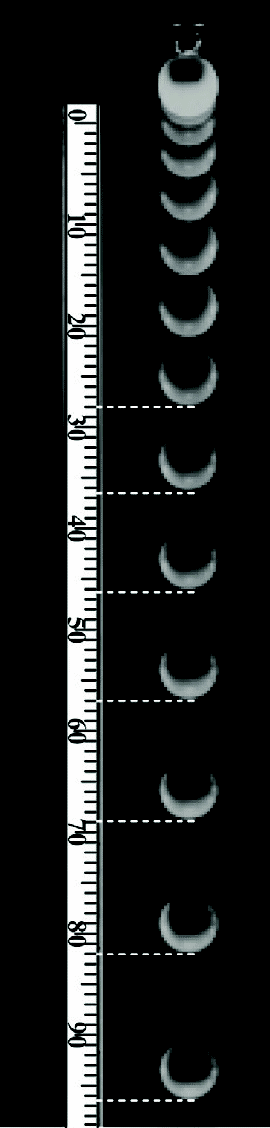
\includegraphics{2-21.pdf}
  \caption{}\label{fig:2-21}
\end{minipage}
\end{figure}

如果导线的运动方向跟导线本身垂直,但跟磁力线方向有一个夹角 $\theta$(\cref{fig:2-21}),我们可以把速度 $v$ 分解为两个分量:垂直于磁力线的分量 $v_1=v\sin\theta$,平行于磁力线的分量 $v_2=v\cos\theta$。
后者不切割磁力线,不产生感生电动势。
前者切割磁力线,产生的感生电动势为 $\mathcal{E}=Bl v_1$,而 $v_1=v\sin\theta$,所以
\begin{equation}
  \label{eq:induced_electromotive_force_crossproduct}
  \mathcal{E}=Bl v\sin\theta.
\end{equation}

可见,\emph{导线切割磁力线时产生的感生电动势的大小,跟磁感应强度 $B$、导线长度 $l$、运动速度 $v$ 以及运动方向和磁力线方向的夹角 $\theta$ 的正弦 $\sin\theta$ 成正比}。

在国际单位制中,\cref{eq:induced_electromotive_force,eq:induced_electromotive_force_crossproduct} 两式中的 $\mathcal{E}$、$B$、$l$、$v$ 的单位分别用伏、特、米、米/秒。
同学们可以自己证明,公式等号两边的单位是一致的,即 $\qty{1}{V}=\qty{1}{T}\times \qty{1}{m}\times\qty{1}{m/s}$。

\begin{example}
  在\cref{fig:2-20} 中,设匀强磁场的磁感应强度 $B=\qty{0.1}{T}$,导体 $ab$ 的长度 $l=\qty{40}{cm}$,向右匀速运动的速度 $v=\qty{5.0}{m/s}$,框架的电阻不计,导体 $ab$ 的电阻 $R=\qty{0.5}{\ohm}$。试求:
  \begin{enumerate}
    \item 感生电动势和感生电流的大小;
    \item 感生电流和感生电动势的方向。
  \end{enumerate}
\end{example}

\begin{solution}
\begin{enumerate}
    \item 线框中的感生电动势
\[\mathcal{E}=Blv=0.1\times0.4\times5.0=\qty{0.2}{V}.\]    
线框中的感生电流
\[I=\frac{\mathcal{E}}{R}=\frac{0.2}{0.5}=\qty{0.4}{A}.\]

\item 利用楞次定律或右手定则,都可以确定出线框中的感生电流方向是沿反时针方向流动的,在导体 $ab$ 中是由 $b$ 指向 $a$。 导体 $ab$ 中的感生电动势的方向和感生电流的方向一致,也是由 $b$ 指向 $a$。
\end{enumerate}
\end{solution}
   
\begin{Reading}{寻找磁单极子}
人们早就发现电和磁有很多相似之处。
例如,带电体的周围有电场,磁体的周围有磁场。
同种电荷互相推斥,异种电荷互相吸引;同名磁极互相推斥,异名磁极互相吸引。
然而尽管电与磁有这样多的相似之处,它们却不是完全相似的。
在电现象里,有电荷,正、负电荷可以单独存在。
在磁现象里却没有发现磁荷,南北极也不能单独存在。
一块磁体,无论把它分得多么小,总是有南极和北极。

但是,1931 年,著名的英国物理学家狄拉克从理论上预言了存在着只有一个磁极的粒子——磁单极子。
根据磁单极子的理论,电和磁之间的相似将更加完美。
理论的动人前景,吸引了一批物理学家,用各种方法,在岩石中,在宇宙射线(即从字宙空间飞来的粒子)中,在加速器实验中,去寻找磁单极子。
但是,半个世纪的时间过去了,并没有找到磁单极子。
因此,人们推测,磁单极子可能是在宇宙形成初期产生的,残存下来的为数较少,而且分散在广漠的宇宙之中,要找到它不是很容易的。

\medskip\noindent
\begin{minipage}{0.72\linewidth}\parindent2em
1982 年,美国的一位物理学家卡布莱拉宣布,在他的实验仪器中通过了一个磁单极子。
他的实验所根据的原理就是电磁感应现象。
仪器的主要部分是一个由超导体做成的线圈。
超导体的电阻为零,一个很微小的电动势就可以在超导线圈中引起感生电流,而且这个电流将长期维持下去,并不减弱。
设想有一个磁单极子穿过超导线圈(\cref{fig:2-22}),穿过超导线圈的磁通量将发生改变,而且引起的感生电动势的方向不变,于是在超导线圈中将引起稳定的电流。
1982 年 2 月 14 日,这位物理学家发现在超导线圈中出现了稳定的电流,经过周密分析,实验所得的数据跟磁单极子理论符合得很好,因而认定这是磁单极子穿过了超导线圈。
不过由于以后没有重复观察到那次实验中观察到的现象,所以这一事例还不能确证磁单极子的存在。
\end{minipage}\hfill
\begin{minipage}{0.23\linewidth}\centering
  \begin{figurehere}
    \begin{minipage}{\linewidth}\centering
      \includegraphics{2-22.pdf}
      \caption{}\label{fig:2-22}
    \end{minipage}
  \end{figurehere}
\end{minipage}

\medskip
目前,寻找磁单极子的实验还在进行中,有关磁单极子的理论,探讨得更深入了。
如果磁单极子确实存在,现在的电磁理论就要做重大的修改,对整个物理学基础理论的发展,也将产生重大的影响。
\end{Reading}

\begin{Practice}
\begin{question}
  \item 下列说法哪个正确?
  \begin{tasks}
    \task 电路中感生电动势的大小,跟穿过这一电路的磁通量成正比;
    \task 电路中感生电动势的大小,跟穿过这一电路的磁通量的变化量成正比;
    \task 电路中感生电动势的大小,跟穿过这一电路的磁通量的变化率成正比;
    \task 电路中感生电动势的大小,跟单位时间内穿过这一电路的磁通量的变化量成正比。
  \end{tasks}
  \item 试证明:$\qty{1}{V}=\qty{1}{Wb/s}$;$\qty{1}{V}=\qty{1}{T}\cdot \qty{1}{m}\cdot \qty{1}{m/s}$。
  \item  长 \qty{5}{cm} 的导线在 \qty{0.02}{T} 的匀强磁场中运动,运动的方向跟磁力线垂直,运动的速率 $v=\qty{0.1}{m/s}$,求感生电动势。
  \item 在 \qty{0.4}{T} 的匀强磁场中,长度为 \qty{25}{cm} 的导线以 \qty{6}{m/s} 的速率做切割磁力线的运动,运动方向跟磁力线成 \ang{30} 角,并跟导线本身垂直。求感生电动势。
  \item 50 匝的线圈,穿过它的磁通量的变化率为 \qty{0.5}{Wb/s},求感生电动势。
  \item 有一个 1000 匝的线圈,在 \qty{0.4}{s} 内穿过它的磁通量从 \qty{0.02}{Wb} 增加到 \qty{0.09}{Wb},求线圈中的感生电动势,如果线圈的电阻是 \qty{10}{\ohm},把它跟一个电阻为 \qty{990}{\ohm} 的电热器串联组成闭合电路时,通过电热器的电流是多大?
  \item \cref{fig:2-23} 是法拉第做成的世界上第一个发电机模型的原理图。把一个铜盘放在磁场里,使磁力线垂直穿过铜盘;转动铜盘,就可以获得持续的电流。试解释其作用原理。
  \begin{figurehere}
    \begin{minipage}{\linewidth}\centering
      \includegraphics{2-23.pdf}
      \caption{}\label{fig:2-23}
    \end{minipage}
  \end{figurehere}
\end{question}
\end{Practice}

\section{电磁感应现象中能量的转化}

在电磁感应现象中,产生感生电动势的那部分导体相当于电源。
\cref{fig:2-1} 中的导体 $AB$,\cref{fig:2-2} 中的螺线管,\cref{fig:2-3} 中的螺线管 $B$,对外电路来说,都相当于电源。
如果使外电路闭合,在感生电动势的作用下就有了感生电流。
这时电流做功消耗了电能。
我们知道,能量不能无中生有,只能从一种形式转化成另一种形式,各种电源都是把其他形式的能转化成电能的装置。
电磁感应现象中的电能是怎样转化而来的呢?

在\cref{fig:2-2} 所示的实验中,按照楞次定律,感生电流总要阻碍磁铁相对于螺线管的运动。
把磁铁移近螺线管时,磁铁受到斥力,必须有外力克服这种斥力做功,才能把磁铁移近。
让磁铁离开螺线管时,磁铁受到引力,也必须有外力克服这种引力做功,才能使磁铁离开。
外力克服这种电磁的引力或斥力做功的过程中,外部的机械能就转化为感生电流的电能。
在\cref{fig:2-1} 中,导线 $ab$ 切割磁力线运动时,按照楞次定律,感生电流也要阻碍导线相对于磁铁的运动。
例如当导线 $ab$ 向右运动时,感生电流在磁场中所受的安培力,方向是向左的,外力克服安培力做功的过程中,外部的机械能就转化为感生电流的电能。
从这里我们也看到,楞次定律跟能的转化和守恒定律是相符的。
我们在初中学过,发电机是利用电磁感应现象制成的。
发电机就是把机械能转化成电能的装置。

现在让我们进一步定量地从能量守恒的观点来研究\cref{fig:2-20} 的实验,并由此推出上一节给出的\cref{eq:induced_electromotive_force}。
当导线 $ab$ 向右运动时,感生电流 $I$ 在磁场中所受的安培力,方向是向左的,大小为 $F=Il B$。
为了保持导线 $ab$ 匀速向右运动,加在导线 $ab$ 上向右的外力,大小应该跟安培力 $F$ 相等。
在 $\Delta t$ 时间内外力克服安培力所做的功为
\[W=Fv\Delta t=Il Bv\Delta t.\]
设感生电动势为 $\mathcal{E}$,在时间 $\Delta t$ 内感生电流所做的功为
\[W'=\mathcal{E}I\Delta t.\]
根据能量守恒定律,这两个功一定相等,因此
\[\mathcal{E}I\Delta t=Il B v \Delta t.\]
由此就得到上节给出的\cref{eq:induced_electromotive_force}:
\[\mathcal{E}=Bl v.\]

可见,法拉第电磁感应定律跟能的转化和守恒定律也是相符的。

\begin{example}
继续做上一节的例题,求
\begin{enumerate}
    \item 使导体 $ab$ 向右匀速运动所需的外力;
    \item 外力做功的功率;
    \item 感生电流的功率。
\end{enumerate}
\end{example}

\begin{solution}
    \begin{enumerate}
        \item 外力跟感生电流所受的安培力平衡,因此外力的大小为
        \[F=Il B=0.4\times0.4\times0.1=\qty{0.016}{N}.\]
        \item 外力做功的功率为
        \[P=Fv=0.016\times5.0=\qty{0.08}{W}.\]
        \item 感生电流的功率为
        \[P'=\mathcal{E}I=0.2\times0.4=\qty{0.08}{W}.\]
    \end{enumerate}
\end{solution}

我们看到,$P=P'$,这正是能量守恒定律所要求的。
线框是纯电阻电路,电流的功全部用来生热,所以热功率 $I^2R$ 也应该等于 $P$ 或 $P'$。
简单的计算指出,情况正是这样的。

\begin{Practice}
\begin{question}
    \item 在\cref{fig:2-20} 中,以一定速度向右拉动导体 $ab$,如果导体 $ab$ 的电阻增大,在相同的时间里,外力做的功是增大还是减小?为什么?
    \item 在\cref{fig:2-20} 中,是快拉还是慢拉所需的功率多?为什么?
    \item 在\cref{fig:2-20} 中,导体 $ab$ 刚开始受到恒力拉动时,它做什么运动?随后它的运动情况将如何变化?感生电动势和感生电流将如何变化?外力做的功产生了哪些效果?如果在导体 $ab$ 还没拉出磁场时停止外力,情况又将怎样?(不考虑摩擦和空气阻力)
\end{question}
\end{Practice}

\section{直流电动机的反电动势}
\subsection{直流电动机}
我们在初中已经学过直流电动机的构造原理,这里简单复习一下。
电动机是把电能转化为机械能的装置,用直流电源供电的电动机叫做直流电动机。
直流电动机是利用通电线圈在磁场里转动的原理制成的。
我们知道,通电线圈在磁场中要受到力矩的作用而发生转动。
但线圈中通入一定方向的电流时,线圈转到它的平面跟磁力线垂直的平衡位置时,就会停下来。
因此,直流电动机中装有换向器(\cref{fig:2-24}),它由两个铜制的半环组成。
有了换向器,线圈转到平衡位置时可以自动改变线圈里的电流方向,线圈就可以不停地转动下去了。
\begin{figure}
\includegraphics{2-24.pdf}
\caption{直流电动机的模型}\label{fig:2-24}
\end{figure}

\subsection{直流电动机的反电动势}

电动机的线圈在磁场里转动时,线圈导线切割磁力线,所以在线图中必然要产生感生电动势,由楞次定律知道,这个感生电动势的方向跟使线圈转动的电流方向相反,因此也跟外加电压的方向相反,通常把这个电动势叫做\Concept{反电动势}。
电动机的线圈转动得越快,线圈导线切割磁力线越快,反电动势就越大。
显然,只有线圈转动时,才有反电动势。

如果用 $\mathcal{E}$ 表示反电动势,$U$ 表示外加电压,$R$ 表示线圈的电阻,那么,电动机工作时的电流强度 $I$ 就是
\begin{equation}
  \label{eq:closed_electric_current}
  I=\frac{U-\mathcal{E}}{R}.
\end{equation}
\cref{eq:closed_electric_current} 可以改写为
\begin{equation}
  \label{eq:closed_electric_voltage}
  U=\mathcal{E}+IR.
\end{equation}
上式表明:电路中有反电动势存在时,加在电路两端的电压 $U$ 等于反电动势 $\mathcal{E}$ 跟线圈电阻上损失的电压 $IR$ 之和。

如果用 $I$ 乘\cref{eq:closed_electric_voltage} 的各项就得到
\begin{equation}
  \label{eq:input_power}
  UI=\mathcal{E}I+I^2R.
\end{equation}
上式中的 $UI$ 是电路供给电动机的功率(输入功率),$\mathcal{E}I$ 是转化为机械能的功率(输出功率),$I^2R$ 是在电动机线圈上损失的热功率。
上式表示,电路供给电动机的功率等于转化为机械能的功率与线圈上损失的热功率之和。
可见能的转化和守恒定律对直流电动机是完全适用的。
从这里我们也看到电功和电热的区别。
在直流电动机中,由于存在着反电动势,有一部分电能转化为机械能,电功并不等于电热,而是大于电热。

在外加电压 $U$ 一定的情况下,电动机的输入功率并不是在任何情况下都相同。
电动机带动负载工作时,线圈受到两个力矩的作用。
一个是通电线圈在磁场中受到的力矩,它使线圈转动,叫做动力矩;一个是负载和机械摩擦所造成的力矩,它阻碍线圈转动,叫做阻力矩。
当动力矩和阻力矩平衡时,电动机匀速转动。
当负载增加时阻力矩增大,线圈的转速减小,反电动势随着减小。从\cref{eq:closed_electric_current} 知道,这时电流强度增大;从\cref{eq:input_power} 知道,这时输入功率也增大。
可见,电动机的输入功率是随着负载的增加而增大的。
线圈中的电流强度增大时,电动机的动力矩也增大,当动力矩增大到和阻力矩平衡时,电动机就在较小的转速下重新做匀速转动。

\section{自感}
在电磁感应现象中,有一种叫做自感现象的特殊情形,现在来研究这种现象。
\subsection{自感现象}
在\cref{fig:2-25} 所示的实验中,先合上开关 $K$,调节变阻器 $R$ 的电阻,使同样规格的两个灯泡 $A_1$ 和 $A_2$ 的明亮程度相同。
再调节变阻器 $R_1$ 使两个灯泡都正常发光,然后断开开关 $K$。
\begin{figure}
  \begin{minipage}[b]{0.48\linewidth}\centering
    \includegraphics{2-25.pdf}
    \caption{}\label{fig:2-25}
  \end{minipage}
  \begin{minipage}[b]{0.48\linewidth}\centering
    \includegraphics{2-26.pdf}
    \caption{}\label{fig:2-26}
  \end{minipage}
\end{figure}

再接通电路时可以看到,跟变阻器 $R$ 串联的灯 $A_2$ 立刻正常发光,而跟有铁芯的线圈$L$ 串联的灯 $A_1$ 却是逐渐亮起来的。
为什么会出现这样的现象呢?
原来,在接通电路的瞬间,电路中的电流增大,穿过线圈 $L$ 的磁通量也随着增加,根据电磁感应定律,线圈中必然会产生感生电动势,这个感生电动势阻碍线圈中电流的增大。
所以通过 $A_1$ 的电流只能逐渐增大,灯 $A_1$ 只能逐渐亮起来。

现在再来做\cref{fig:2-26} 的实验,把灯泡 $A$ 和带铁芯的电阻较小的线圈 $L$ 并联接在直流电路里。
接通电路,灯 $A$ 正常发光后,再断开电路,这时可以看到,灯 $A$ 要过一会儿才熄灭。
为什么会出现这种现象呢?
这是由于电路断开的瞬间,通过线圈的电流突然减弱,穿过线圈的磁通量也就很快地减少,因而在线圈中产生感生电动势。
虽然这时电源已经断开,但线圈 $L$ 和灯泡 $A$ 组成了闭合电路,在这个电路中有感生电流 $I$ 通过,所以灯泡不会立即熄灭。

从上述两个实验可以看出,当导体中的电流发生变化时,导体本身就产生感生电动势,这个电动势总是阻碍导体中原来电流的变化的。
这种由于导体本身的电流发生变化而产生的电磁感应现象,叫做\Concept{自感现象}。
在自感现象中产生的感生电动势,叫做\Concept{自感电动势}。

\subsection{自感系数}
自感电动势跟其他感生电动势一样,是跟穿过线圈的磁通量的变化率 $\Delta\phi/\Delta t$ 成正比的。
我们知道,磁通量 $\phi$ 跟磁感应强度 $B$ 成正比,$B$ 又跟产生这个磁场的电流 $I$ 成正比。
所以 $\phi$ 跟 $I$ 成正比,$\Delta \phi$ 跟 $\Delta I$ 也成正比,由此可知自感电动势 $\mathcal{E}=\Delta\phi/\Delta t$ 跟 $\Delta I/\Delta t$ 成正比,即
\[\mathcal{E}=L\frac{\Delta I}{\Delta t}.\]
式中的比例恒量 $L$ 叫做线圈的\Concept{自感系数},简称自感或电感,它是由线圈本身的特性决定的。
线圈越长,单位长度上的匝数越多,截面积越大,它的自感系数就越大。
另外,有铁芯的线圈的自感系数,比没有铁芯时要大得多。
对于一个现成的线圈来说,自感系数是一定的。

自感系数的单位是\Concept{亨利},简称亨,国际符号是 \unit{H}。
如果通过线圈的电流强度在 \qty{1}{s} 内改变 \qty{1}{A} 时产生的自感电动势是 \qty{1}{V},这个线圈的自感系数是 \qty{1}{H}。所以
\[\qty{1}{H}=\qty{1}{V.s/A}.\]

常用的较小单位有毫亨(\unit{mH})和微亨(\unit{\micro H})。
\[\qty{1}{mH}=\qty{e-3}{H},\qquad \qty{1}{\micro H}=\qty{e-6}{H}.\]

\section{自感现象的应用}
自感现象在各种电器设备和无线电技术中有广泛的应用。
日光灯的镇流器就是利用线圈自感现象的一个例子。

\cref{fig:2-27} 是日光灯的电路图,它主要是由灯管、镇流器和起动器组成的。
镇流器是一个带铁芯的线圈。
起动器的构造如\cref{fig:2-28} 所示,它是一个充有氖气的小玻璃泡,里面装有两个电极,一个固定不动的静触片和一个用双金属片制成的 U 形触片。
灯管内充有稀薄的水银蒸气。
当水银蒸气导电时,就发出紫外线,使涂在管壁上的荧光粉发出柔和的白光。
由于激发水银蒸气导电所需的电压比 \qty{220}{V} 的电源电压高得多,因此,日光灯在开始点燃时需要一个高出电源电压很多的瞬时电压。
在日光灯点燃后正常发光时,灯管的电阻变得很小,只允许通过不大的电流,电流过强就会烧毁灯管,这时又要使加在灯管上的电压大大低于电源电压。
这两方面的要求都是利用跟灯管串联的镇流器来达到的。
\begin{figure}
	\begin{minipage}[b]{0.48\linewidth}\centering
		\includegraphics{2-27.pdf}
		\caption{}\label{fig:2-27}
	\end{minipage}
	\begin{minipage}[b]{0.48\linewidth}\centering
		\includegraphics{2-28.pdf}
		\caption{}\label{fig:2-28}
	\end{minipage}
\end{figure}

当开关闭合后,电源把电压加在起动器的两极之间,使氖气放电而发出辉光。
辉光产生的热量使 U 形触片膨胀伸长,跟静触片接触而把电路接通。
于是镇流器的线圈和灯管的灯丝中就有电流通过,电路接通后,起动器中的氖气停止放电,U 形触片冷却收缩,两个触片分离,电路自动断开。
在电路突然中断的瞬间,在镇流器两端产生一个瞬时高电压,这个电压加上电源电压加在灯管两端,使灯管中的水银蒸气开始放电,于是日光灯管成为电流的通路开始发光。
在日光灯正常发光时,由于交流电不断通过镇流器的线圈,线圈中就有自感电动势,它总是阻碍电流变化的,这时镇流器起着降压限流作用,保证日光灯的正常工作。

自感现象也有不利的一面。
在自感系数很大面电流又很强的电路(如大型电动机的定子绕组)中,在切断电路的瞬间,由于电流强度在很短的时间内发生很大的变化,会产生很高的自感电动势,使开关的闸刀和固定夹片之间的空气电离而变成导体,形成电弧。
这会烧坏开关,甚至危及工作人员的安全。
因此,切断这类电路时必须采用特制的安全开关。
常见的安全开关是将开关放在绝缘性能良好的油中,防止电弧的产生,保证安全。

\begin{Practice}
\begin{question}
  \item 制造电阻箱时,要用双线绕法,如\cref{fig:2-29} 所示,这样就可以使自感现象的影响减弱到可以略去的程度,为什么?
  \begin{figurehere}
    \begin{minipage}{\linewidth}\centering
      \includegraphics{2-29.pdf}
      \caption{}\label{fig:2-29}
    \end{minipage}
  \end{figurehere}
  \item 有一个线圈,它的自感系数是 \qty{1.2}{H},当通过它的电流在 \qty{0.005}{s} 内由零增加到 \qty{5.0}{A} 时,线圈中产生的自感电动势多大?
  \item 一个线圈的电流强度在 \qty{0.001}{s} 内有 \qty{0.02}{A} 的变化时,产生 \qty{50}{V} 的自感电动势,求线圈的自感系数,如果这个电路中电流强度的变化率变为 \qty{40}{A/s},自感电动势是多大?
  \item 试证明 $\qty{1}{H}=\qty{1}{\ohm.s}$。
  \item 根据感生电动势 $\mathcal{E}=\dfrac{\Delta \phi}{\Delta t}$ 和 $\mathcal{E}=L\dfrac{\Delta I}{\Delta t}$,证明 $L=\dfrac{\Delta \phi}{\Delta I}$,并说明这个式子的物理意义。
\end{question}
\end{Practice}

\section{涡流}

仔细观察发电机、电动机和变压器,可以看到它们的铁芯都不是整块金属,而是用许多薄的硅钢片叠合而成的。
为什么要这样呢?

原来,把块状金属放在变化的磁场中,或者让它在磁场中运动时,金属块内将产生感生电流。
这种电流在金属块内白成闭合回路,很象水的旋涡,因此叫做涡电流,简称\Concept{涡流}。
整块金属的电阻很小,所以涡流常常很强。

如\cref{fig:2-30} 所示,在块状铁芯上绕绝缘导线,当交流电通过导线时,穿过铁芯的磁通量不断变化,铁芯中就会产生如图中虚线所示的涡流。
块状铁芯中的涡流很强,这将使铁芯大量发热,浪费大量的电能。
因此用整块铁芯的电机和变压器,涡流损失很大,效率很低。

\begin{figure}
	\begin{minipage}[b]{0.48\linewidth}\centering
    \includegraphics{2-30.pdf}
		\caption{}\label{fig:2-30}
	\end{minipage}
	\begin{minipage}[b]{0.48\linewidth}\centering
    \includegraphics{2-31.pdf}
    \caption{}\label{fig:2-31}
	\end{minipage}
\end{figure}

为了减少涡流损失,电机和变压器通常用涂有绝缘漆的薄硅钢片叠压制成的铁芯,如\cref{fig:2-31} 所示。
这样涡流被限制在狭窄的薄片之内,回路的电阻很大,涡流大为减弱,从而使涡流损失大大降低。
铁芯采用硅钢片,是因为这种钢比普通钢的电阻率大,可以进一步减少涡流损失。
硅钢的涡流损失只有普通钢的 $1/5$~$1/4$。

在各种电机、变压器中,涡流是有害的,我们要采取各种办法来减弱它。
但是涡流也是可以利用的,下面举两个例子。

\medskip\noindent
\begin{minipage}{0.6\linewidth}\parindent2em
  \cref{fig:2-32} 是冶炼金属的高频感应炉的示意图,这种电炉就是利用涡流来熔化金属的。
  冶炼锅内装入被冶炼的金属,让高频交流电通过线圈,被冶炼的金属中就产生很强的涡流,从而产生大量的热使金属熔化。
  这种冶炼方法速度快,温度容易控制,并能避免有害杂质混入被冶炼的金属中,因此适于冶炼特种合金和特种钢。
\end{minipage}\hfill
\begin{minipage}{0.35\linewidth}\centering
  \begin{figurehere}
    \includegraphics{2-32.pdf}
    \caption{}\label{fig:2-32}
  \end{figurehere}
\end{minipage}

\medskip
电学测量仪表要求指针的摆动很快停下来,以便可以迅速读出读数。
我们在\cref{chp:magnetic_field}讲的电流表的线圈要绕在铝框上,铝框就是起这个作用的。
原来,当被测电流通过线圈时,线圈带动指针和铝框一起转动。
铝框在磁场中转动时产生涡流,磁场对这个涡流的作用力阻碍它们的摆动,于是使指针很快地稳定指到读数位置上。

\begin{Practice}
\begin{question}
  \item 如\cref{fig:2-33} 所示,$A$ 是可以在电磁铁两磁极间摆动的铝片(或铜片)。电磁铁线围没有通电时,铝片可以摆动较长时间才停下来。电磁铁线圈通电时,铝片很快就会停下来。解释这个现象。
    
  这种现象叫做电磁阻尼,在实际中有很多应用。课文中讲的,使电学测量仪表的指针很快地停下来,就是电磁阻尼的应用。电磁阻尼还常用于电气机车的电磁制动器中。
  \begin{figurehere}
    \begin{minipage}{\linewidth}
    \begin{minipage}[b]{0.45\linewidth}\centering
      \includegraphics{2-33.pdf}
      \caption{电磁阻尼}\label{fig:2-33}
    \end{minipage}
    \begin{minipage}[b]{0.5\linewidth}\centering
      \includegraphics{2-34.pdf}
      \caption{电磁驱动}\label{fig:2-34}
    \end{minipage}
    \end{minipage}
  \end{figurehere}
  \item 如\cref{fig:2-34} 所示,把蹄形磁铁的两极靠近一个金属圆盘,但不接触。当磁铁绕轴转动时,圆盘也绕轴转动起来,解释这个现象。

  这种现象叫做电磁驱动,在实际中也有很多应用,下一章要讲的感应电动机就是利用这个道理驱动的。家庭中用的电度表,汽车上用的电磁式速度表,也利用这种电磁驱动。
\end{question}
\end{Practice}

\begin{Review}
\begin{question}
  \item 什么是电磁感应现象?什么是感生电流?产生感生电流的条件是什么?
  \item 楞次定律的内容是什么?应用楞次定律判定感生电流方向的步骤是怎样的?怎样用右手定则来判断感生电流的方向?
  \item 什么是感生电动势?法拉第电磁感应定律的内容是什么?写出计算单匝线圈和 $n$ 匝线圈的感生电动势的公式,写出导线切割磁力线运动时计算感生电动势的公式。
  \item 在电磁感应现象中能量是怎样转化的?为什么说楞次定律和法拉第电磁感应定律都跟能的转化和守恒定律是相符的?
  \item 什么是直流电动机的反电动势?在直流电动机中能的转化情况是怎样的?
  \item 什么是自感现象?什么是自感系数?写出计算自感电动势的公式。
  \item 什么是涡流?为什么发电机、电动机和变压器的铁芯要用许多相互绝缘的簿硅钢片叠合起来制成?
\end{question}
\end{Review}

\begin{Exercise}
\begin{question}
  \item 在\cref{fig:2-35} 中,条形磁铁以速度 $v$ 向螺线管靠近,下面哪种说法是正确的:
  \begin{figurehere}
    \begin{minipage}[b]{0.38\linewidth}\centering
      \includegraphics{2-35.pdf}
      \caption{}\label{fig:2-35}
    \end{minipage}
    \begin{minipage}[b]{0.58\linewidth}\centering
      \includegraphics{2-36.pdf}
      \caption{}\label{fig:2-36}
    \end{minipage}
  \end{figurehere}
  \begin{tasks}
    \task 螺线管中不产生感生电流;
    \task 螺线管中产生感生电流,方向如\cref{fig:2-35} 所示;
    \task 螺线管中感生电流的方向与图中所示的方向相反。
  \end{tasks}
  \item 在\cref{fig:2-36} 中,线圈 $M$ 和线圈 $P$ 绕在同一铁芯上。
  \begin{tasks}
    \task 当合上电键 $K$ 的一瞬时,线圈 $P$ 里有没有感生电流?
    \task 当线圈 $M$ 里有稳恒电流通过时,线圈 $P$ 里有没有感生电流?
    \task 当断开电键 $K$ 的一瞬时,线圈 $P$ 里有没有感生电流?
  \end{tasks}
  在上面三种情况里,如果线圈 $P$ 里有感生电流,指出线圈 $P$ 的哪一端是 $N$ 极。
  \item 宇航员飞到某一个不熟悉的行星上,他们想用一只灵敏电流表和一个线圈来探测一下行星周围是否有磁场,应当怎样办?
  \begin{figurehere}
    \begin{minipage}{\linewidth}\centering
      \includegraphics{2-37.pdf}
      \caption{}\label{fig:2-37}
    \end{minipage}
  \end{figurehere}
  \item 如\cref{fig:2-37} 所示,在匀强磁场中有一个线圈。
  \begin{tasks}
    \task 当线圈分别以 $P_1$ 和 $P_2$ 为轴按逆时针方向转动时(如图中箭头所示),感生电流的方向各是什么?
    \task 当转速恒定时,线圈以 $P_1$ 和 $P_2$ 为轴转动时,两种情况下感生电流的大小有何关系?
    \task 当转速恒定时,感生电动势的大小跟线圈面积有何关系?
    \task 设磁感应强度 $B$ 为 \qty{1.5}{T},$AB$ 为 \qty{10}{cm},$BC$为 \qty{4}{cm},转速为每秒 $120/2\uppi$ 转,分别求出以 $P_1$ 和 $P_2$ 为转轴时感生电动势的最大值。
  \end{tasks}
  \item 如\cref{fig:2-38} 所示,在磁感应强度为 \qty{0.5}{T} 的匀强磁场中,让长为 \qty{0.2}{m}的导体 $AB$ 在无摩擦的框架上以 \qty{5}{m/s} 的速度向右滑动,如果 $R_1=R_2=\qty{2}{\ohm}$,其他导线的电阻不计,外力做功的功率有多大?感生电流的功率有多大?在电阻 $R_1$ 和 $R_2$ 上消耗的功率有多大?验证一下:能的转化是否符合守恒定律?
  \item 如\cref{fig:2-39} 所示,让铜线圈 $A$ 自由落下,并通过一段有匀强磁场的空间,试定性说明线圈的运动情况。(不考虑空气阻力)
  \begin{figurehere}
    \begin{minipage}[b]{0.48\linewidth}\centering
      \includegraphics{2-38.pdf}
      \caption{}\label{fig:2-38}
    \end{minipage}
    \begin{minipage}[b]{0.48\linewidth}\centering
      \includegraphics{2-39.pdf}
      \caption{}\label{fig:2-39}
    \end{minipage}
  \end{figurehere}
  \item 弹簧上端固定,下端悬挂一根磁铁。将磁铁抬到某一高度后放开,磁铁能上下振动较长时间才停下来。如果在磁铁下端放一个固定的闭合线圈使磁铁上下振动时穿过它(\cref{fig:2-40}),磁铁就会很快地停下来,试用能量观点来解释这个现象。
  \begin{figurehere}
    \begin{minipage}[b]{0.48\linewidth}\centering
      \includegraphics{2-40.pdf}
      \caption{}\label{fig:2-40}
    \end{minipage}
    \begin{minipage}[b]{0.48\linewidth}\centering
      \includegraphics{2-41.pdf}
      \caption{}\label{fig:2-41}
    \end{minipage}
  \end{figurehere}
  \item \cref{fig:2-41} 是生产中常用的一种延时继电器的示意图。铁芯上有两个线圈 $A$ 和 $B$。线圈 $A$ 跟电源连接,线圈 $B$ 的两端接在一起,构成一个闭合电路,在拉开电键 $K$ 的时候,弹簧 $S$ 并不能立即将衔铁 $D$ 拉起,从而使触头 $C$(连接工作电路)立即离开,过一段短时间后触头 $C$ 才能离开;延时继电器就是这样得名的,试说明这种继电器的原理。
  \begin{figurehere}
    \begin{minipage}{\linewidth}\centering
      \includegraphics{2-42.pdf}
      \caption{}\label{fig:2-42}
    \end{minipage}
  \end{figurehere}
  \item 普通磁带录音机是用同一个磁头来录音和放音,磁头结构如\cref{fig:2-42} 所示,在一个环形铁芯上绕着一个线圈,录音时,磁头线圈跟微音器相连,放音时,磁头线圈改为跟扬声器相连,微音器的作用是把声音的变化转变为线圈中电流的变化,扬声器的作用是把线圈中电流的变化转化为声音的变化,铁芯有个缝隙,工作时磁带就贴着这个缝隙移动。磁带上涂有一层磁粉,磁粉能被磁化,并且留下剩磁。

  根据学过的知识先自己想一想录、放音的原理;再找有关的书或文章看看自己想得对不对,然后把录、放音的基本原理简明扼要地写下来。
  \item 如\cref{fig:2-43} 所示,电源的电动势 $\mathcal{E}=\qty{1.5}{V}$,内电阻 $r=\qty{0.5}{\ohm}$,$AB=\qty{0.5}{m}$,$AB$ 的电阻 $R=\qty{0.1}{\ohm}$,框架的电阻不计,磁感应强度为 \qty{0.5}{T},金属框对 $AB$ 的滑动摩擦力为 \qty{0.25}{N}。
  \begin{tasks}
    \task 分析一下,当电键 $K$ 闭合后,会发生哪些电磁现象?
    \task 当 $AB$ 的速度达到稳定时(即速度为最大时),电路中的电流强度是多大?
    \task $AB$ 的最大速度是多少?
    \task 这时电源消耗的电能转化为什么形式的能?通过计算验证一下:能的转化是否符合守恒定律?
  \end{tasks}
  \begin{figurehere}
    \begin{minipage}{\linewidth}\centering
      \includegraphics{2-43.pdf}
      \caption{}\label{fig:2-43}
    \end{minipage}
  \end{figurehere}
\end{question}
\end{Exercise}